%----------------------------------------------------------------------------
\chapter{A tekintetkövetésről}\label{sect:tekintetkovetes}
%----------------------------------------------------------------------------

A tekintetkövető rendszer fejlesztésének megkezdése előtt számos elméleti és gyakorlati szempont veendő figyelembe, hogy a rendszer által nyújtott kritériumok a lehető legjobban közelítsék az elvártat. Nem kerülhető meg az általános technikák, vagy már meglévő megoldások áttekintése a szakirodalomból, aminek segítségével képet alkothatunk a kutatási téma jelenlegi állásáról, és a gyakorlati szempontok figyelembe vételével dönthetjük el, hogy mely módszer mellett tesszük le végül a voksunkat.

\bigskip

A fejezet \sectref{modszerek} szakaszában mindenekelőtt a jelenleg elérhető tekintetkövetési módszereket veszem górcső alá, majd hasonlítom össze őket, hogy kellően megalapozott döntést hozhassak a később felhasználni kívánt technikával kapcsolatban. 

%,,,,,,,,,,,,,,,,,,,,,,,,,,,,,,,,,,,,,,,,,,,,,,,,,,,,,,,,,,,,,,,,,,,,,,,,,,,,
\section{Tekintetkövetési módszerek}\label{sect:modszerek}
%,,,,,,,,,,,,,,,,,,,,,,,,,,,,,,,,,,,,,,,,,,,,,,,,,,,,,,,,,,,,,,,,,,,,,,,,,,,,

Bár már lassan másfél évtizedes, a témában mégis hiánypótló munka Arne John Glenstroupnak és Theo Engell-Nielsennek, a dán Københavns Universitet (Koppenhágai Egyetem) hallgatóinak diplomamunkája \cite{eye_media}. Dolgozatuk jelen szempontból fontos második fejezetét a modern tekintetkövetési technikák bemutatásának és összehasonlításának szentelik, meglátásaik pedig mind a mai napig helytállóak.

\bigskip

Ebben a szakaszban főleg az ő munkájuk alapján szeretném összefoglalni a tekintet követésére felhasználható technikákat, néhol a lényeg kiemelésével, ahol pedig szükséges, a hivatkozott cikk keletkezése óta az idő múlásával érvénytelenné vált adatok, paraméterek aktualizálásával.

%............................................................................
\subsection{Az ideális tekintetkövető}\label{sect:idealis}
%............................................................................

Manapság számos módszer kínálkozik a tekintet követésére. De mégis milyen követelményeket kell teljesíteni az ,,ideális'' tekintetkövetőnek? Scott és Findlay 1993-as munkájukban \cite{scott} Hallett eredményeit \cite{hallett} figyelembe véve meghatározták az ideális tekintetkövető eszköz (vagy rendszer) paramétereit és tulajdonságait.

Ezek szerint az ideális tekintetkövető eszköznek a következő 12 pont által támasztott követelményeket kell teljesítenie:

\begin{enumerate}[a.]
 \item az arc és a fejrégió könnyen hozzáférhető maradjon
 \item ne legyen fizikailag kapcsolatban a vizsgált személlyel
 \item ha szükséges, képes legyen stabilizálni a kapott eredményeket
 \item a rendszer \emph{pontossága} néhány százalékos (1--2 szögperces) eltérést engedjen meg
 \item támogasson legalább egy szögperces \emph{felbontást} másodpercenként, hogy a szempozíció legkisebb változása is követhető legyen; a felbontásnak csak az érzékelő eszköz zaja szabjon határt
 \item támogasson kellően széles \emph{dinamika-tartományt} a szem mozogásainak leképezéséhez
 \item a rendszer időbeli dinamikája legyen megfelelő (jó erősítés, kis fázistolás)
 \item nyújtson \emph{valósidejű} válaszidőt
 \item legyen \emph{invariáns} mindhárom forgási és eltolási szabadságfokra
 \item egyszerűen kiterjeszthető legyen mindkét szem feldolgozására (\emph{binokuláris} vizsgálat)
 \item \emph{kompatibilis} meglévő legyen fej- és testfelvételek használatával
 \item tesztalanyok széles skáláján (pl. nem, kor, rassz szerint, vagy szemüvegesek és szemüveg nélküliek körében) használható legyen
\end{enumerate}

A fent felsorolt követelmények valóban az ideális esetet testesítik meg. Sokszor egy követelmény enyhítésével, vagy figyelmen kívül hagyásával más követelmények kielégítése jelentősen egyszerűsödik. Ha például a \emph{b.} pont szerinti fizikai kontaktust mégis megengedjük, rögzíthetjük a követésre használt kamerát a vizsgálni kívánt alany fejéhez (természetesen kellően diszkrét és kényelmes módon). Ebben az esetben a \emph{i.} pont szerinti invariancia biztosítása máris egyszerűbb feladat, mint külső nézőpontból geometriai transzformációk segítségével végezni ugyanezt.

Több más, látszólag egymásnak ellentmondó követelményt is észrevehetünk az ideális tekintetkövető eszköz 12 pontja között. Komoly megoldandó mérnöki feladatot jelent az ütközések feloldásával az ideális eszközt különböző, valós életben használható megoldásokká alakítani.

\bigskip

A gyakorlatban használható tekintetkövetési megoldások egy lehetséges csoportosítása az alábbi elveken működő iránymeghatározásokat tartalmazza:

\begin{enumerate}
 \item a szem felületének (vagy a felület speciális megvilágításának) alapján, optikai elven 
 \item a szem körüli bőrfelület elektromos potenciáljának mérésével
 \item speciális kontaktlencse használatával
\end{enumerate}

Már csekély megfontolással látszik, hogy minden csoportnak vannak előnyei és hátrányai. Például az \emph{1.} csoportba tartozó megoldások igénylik a legkevésbé -- többnyire egyáltalán nem -- a fizikai kontaktust a vizsgált személlyel. Azonban elképzelhető, hogy ennek az az ára, hogy az ebbe a csoportba tartozó megoldások nem veszik fel a versenyt a másik két alapelv szerint fejlesztett rendszerekkel pl. a pontosság, vagy valamely más kritérium tekintetében.

Ennek megfelelően szükség van a lehetőségek számba vételére, értékelésére, majd összehasonlítására, hogy a legmegfelelőbb technikát tudjuk kiválasztani, ha tekintetkövető eszköz (alkalmazás) fejlesztésébe fogunk. A következő szakaszokban ezért röviden ismertetem a fenti kategóriákba eső megoldások alapjait, majd összehasonlítom jellemző tulajdonságaikat, valamint a használatukkal elérhető fontos pontossági- és sebességértékeket.

%............................................................................
\subsection{Optikai elvű követés}\label{sect:optikai}
%............................................................................

Az optikai elvű követés során -- a nevéből adódóan -- optikai úton próbáljuk meghatározni a tekintet irányát. Ez történhet speciális megvilágítás nélkül, pl. az írisz (pontosabban az írisz és az ínhártya közti határvonal, a limbus), vagy a pupilla követésével.

A másik lehetséges megoldásra a szem speciális, többnyire infravörös fénnyel történő megvilágítása, majd a szemgolyó felületén megjelenő tükröződések, visszaverődések vizsgálata kínálkozik. Az infravörös megvilágítás előnye a látható fénnyel szemben egyrészt az, hogy nem zavarja a vizsgált személyt, nem vonja el a figyelmét, másrészt pedig infraszűrők használatával a látható fény tartományába eső változásokkal a megfelelő körülmények között (lehetőleg kevés napfény a magas infratartalma miatt) invariánssá tehető.

%. . . . . . . . . . . . . . . . . . . . . . . . . . . . . . . . . . . . . .
\subsubsection{Limbuskövetés}\label{sect:limbusz}
%. . . . . . . . . . . . . . . . . . . . . . . . . . . . . . . . . . . . . .

Az írisz és az ínhártya közötti határvonal a többnyire nagy intenzitásváltozás miatt könnyen detektálható lehet. Ugyanakkor meg kell jegyeznünk, hogy az esetek jelentős részében a limbus számottevő része lehet a szemhéjak takarásában. Ennek megfelelően a technika csak vízszintes helyzet és mozgás követésére alkalmas kielégítő pontossággal \cite{scott}.

Klasszikus esetben ez a követési technika a limbus \emph{relatív} fejhez képest helyzetén alapul, ezért a vizsgálat közben a fejmozgások teljes hanyagolását, esetleg a tekintetkövető eszköz fejhez rögzítettségét igényli.

%. . . . . . . . . . . . . . . . . . . . . . . . . . . . . . . . . . . . . .
\subsubsection{Pupillakövetés}\label{sect:pupilla}
%. . . . . . . . . . . . . . . . . . . . . . . . . . . . . . . . . . . . . .

A pupillakövetési technika hasonló az előbb említett limbuskövetéshez, de némi többlet előnyt is magában hordoz. Az egyik ilyen előny, hogy a pupilla közel sincs olyan nagy részben a szemhéjak takarásában, mint a limbus, ennek következtében függőleges irányú követés is megvalósítható lehet. A másik előny, hogy az írisz és a pupilla közti határvonal jóval élesebb, mint az írisz-ínhártya határa, ezért jobb felbontással, pontosabban tudjuk meghatározni a nézeti irányt.

Az előző technikához képest azonban meg kell említeni a felmerülő nehézségeket is. A kontraszt ugyan lehet, hogy nagyobb az írisz-pupilla határon, azonban az intenzitáskülönbség nem olyan jelentős, mint a limbus környezetében. Az sem elhanyagolható szempont, hogy a pupilla átmérője is szükségszerűen kisebb, mint az íriszé, vagyis a forrásnak relatívan nagyobb felbontásúnak kell lennie, hogy azonos pixelnyi méretű pupillát és íriszt detektálhassunk; ellenkező esetben a kisebb abszolút méret a pontosság rovására mehet.

%. . . . . . . . . . . . . . . . . . . . . . . . . . . . . . . . . . . . . .
\subsubsection{Visszaverődés-alapú követés}\label{sect:visszaverodes}
%. . . . . . . . . . . . . . . . . . . . . . . . . . . . . . . . . . . . . .

A szemet (infravörös) fénnyel megvilágítva több tükröződés is megfigyelhető lesz a szemlencse és a szaruhártya határán: ezek az úgynevezett \emph{Purkinje-képek} (lásd \figref{purkinje} ábra).

\begin{figure}[!ht]
\centering
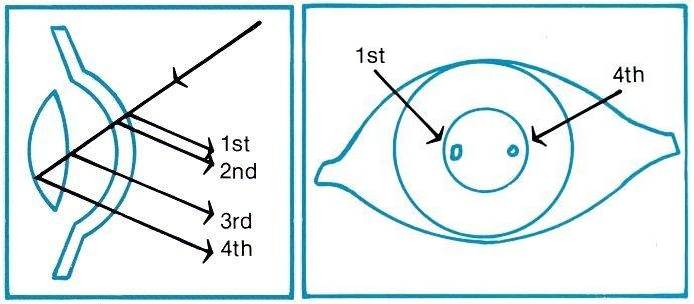
\includegraphics[width=110mm, keepaspectratio]{figures/purkinje_kepek.png}
\caption{A \emph{Purkinje-képek} elhelyezkedése. Forrás: \url{http://bit.ly/YnAowY}}
\label{fig:purkinje}
\end{figure}

Ezen visszavert képek intenzitása sorrendben egyre csökken, az első azonban (közkeletű nevén az úgynevezett \emph{,,csillanás''}, angolul \emph{glint}) még viszonylag egyszerűen detektálható. Infravörös megvilágításban ugyancsak egyszerű a megfelelő kamerával a pupilláról visszavert fény detektálása -- a pupilla a környezeténél jóval nagyobb mértékben veri vissza az infravörös fényt, az infraképen egy ,,fényes'', kontrasztos objektumot alkotva.

A fenti két objektum egymáshoz viszonyított \emph{relatív} helyzetéből következtethetünk a tekintet irányára, ugyanis az első Purkinje-kép világos pontja, illetve a pupilla kontrasztos ellipszise egymással összefüggésben mozdulnak el a fej vagy a szem mozgatásának következtében.

Az előző bekezdésben foglaltakból látszik, hogy a technika nem igényeli a fej mozdulatlanságát, vagy a képfelvevő eszköz fejhez rögzítését. Ezen előnye azonban egy megkötést is magával hordoz: egyszerű algoritmusok segítségével kb. $\pm12$--$15$ foknyi szabadsága van a felhasználónak a fejmozgásokra \cite{scott}, nagyobb mértékű mozgások esetén ugyanis komplexebb matematikai számítások szükségesek a követett objektumok mozgásának modellezéséhez.

\bigskip

A visszaverődés-alapú megoldásokkal rokonítható még az a módszer, amikor szintén az első Purkinje-kép erős visszaverődését detektálva a képen, kivágunk egy viszonylag kicsi (párszor tíz pixel nagyságrendű) részt, a csillanással a középpontban. Az így kapott képről egy neurális hálózat dönti el, hogy milyen nézeti irányhoz tartozik \cite{baluja}.

A neurális hálózatot természetesen be kell tanítani a használhatóság érdekében. A betanítási procedúra első lépéseként tanítóképeket kell generálni, általános esetben pár percet vesz igénybe, ami alatt a követnie kell egy, a képernyőn megjelenő jelzést. A tanítóképek birtokában ezután a hálózat betanítható, ez a jelenlegi technikai szint mellett kb. tíz perces nagyságrendű időt vesz igénybe. Azonban azonos körülmények és tesztszemély esetén a tanítást nem kell máskor újra elvégezni.

A neurális hálózat előnye a betanítás után, használat közben mutatkozik meg leginkább: felépítéséből adódóan a háló nagyon rövid idő alatt ,,döntést tud hozni'', így a valósidejű feldolgozási sebesség kritériuma mindenképpen kielégített lesz. A döntés eredménye ráadásul akár közvetlenül felhasználható: mindössze úgy kell megterveznünk a rendszert, hogy a neurális háló kimenet közvetlenül egy kétdimenziós koordinátát szolgáltasson a felhasznált képernyő koordináta-rendszerében.

A módszer egy másik előnye, hogy nem igényel közeli, nagy felbontású képet a szemrégióról, egy átlagos felbontású kamerával, pl. kartávolságból is elegendő nagyságú lesz a szemrégió. Ennek egyik folyományaként -- hogy nagyobb látószögű képek használhatók -- adódik, hogy viszonylag nagy mozgási szabadsága lehetséges a vizsgált személy fejének tekintetében, anélkül, hogy a kamerát újra kéne pozicionálnunk.

Ennek a szabadságnak azonban ára van: ha a kalibrálási fázis során több fejpozícióból is rögzítettünk tanító képeket, akkor a betanítás után a neurális hálózat jó eséllyel fogja felismerni különböző fejpozíciókban is a tekintet irányát; a mozgási szabadság azonban a pontosság csökkenésével jár. A pontosság egyébként is érzékeny pontja az eljárásnak, ezt pedig éppen úgy növelhetjük, ha tanítás és előhívás közben \emph{nem} engedjük meg, hogy a fejpozíció változzon.

%. . . . . . . . . . . . . . . . . . . . . . . . . . . . . . . . . . . . . .
\subsubsection{Purkinje-képek követése}\label{sect:purkinje}
%. . . . . . . . . . . . . . . . . . . . . . . . . . . . . . . . . . . . . .

Egy további lehetséges optikai elven működő tekintetkövetési technikát mutatott be Müller \emph{et al} 1993-ban \cite{muller}, \emph{,,Kettős Purkinje-kép''} (Dual-Purkinje Image) módszer néven. Az eljárás lényege, hogy a már említett első és negyedik Purkinje-kép egymáshoz viszonyított helyzetéből számítja a tekintet irányát. Megfelelő matematikai modell esetén a módszer rendkívül pontos, azonban a negyedik Purkinje-kép alacsony intenzitása miatt hatványozottan érzékeny a megvilágítási problémákra.

%............................................................................
\subsection{Elektromos potenciál-alapú követés}\label{sect:potencial}
%............................................................................

Az eddigiektől a pupillakövetési probléma egy merőben eltérő megközelítése az \emph{elektro-okulográfia} (EOG). Az eljárásból nyerhető elektro-okulogram rögzítése pl. megismerési és kognitív folyamatok, a vizuális információfeldolgozás, vagy az alvásvizsgálat terén szokásos.

\begin{figure}[!ht]
\centering
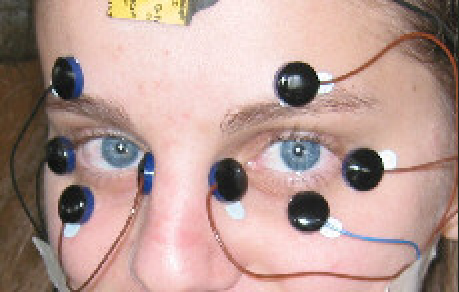
\includegraphics[width=80mm, keepaspectratio]{figures/eog.png}
\caption{Az EOG eljárás elektródái. Forrás: \url{http://bit.ly/13a7IcL}}
\label{fig:eog}
\end{figure}

A módszer a szemgolyó elülső és hátulsó pólusa közötti potenciálkülönbség mérésén alapul, amellyel mind függőleges, mind vízszintes irányban követhető a szem mozgása, de csak körülbelül $1$--$2$ fok pontossággal. A használata azonban korántsem mondható egyszerűnek: az potenciálváltozást érzékelő elektródák (lásd \figref{eog}) miatt szükséges fizikai kontaktuson kívül a rendszer kalibrációja rendkívül hosszadalmas, és hozzáértést igénylő feladat.

%............................................................................
\subsection{Követés speciális kontaktlencse használatával}\label{sect:kontakt}
%............................................................................

A szem helyzetének, ebből közvetve a tekintet irányának számításához speciális kontaktlencséket is használhatunk. Az egyik lehetséges megoldás, hogy a lencse anyagában olyan véseteket alakítanak ki (tipikusan valamilyen könnyen felismerhető mintázatot), amelyek a fénytörés felhasználásával megkönnyítik a szem helyzetének meghatározását.

Ha azonban egy megfelelően kis méretű indukciós tekercset is sikerült a kontaktlencse anyagába ágyazni, akkor a fej körül generált nagyfrekvenciás elektromágneses mezőkkel az tekercs helyzete közvetlenül is könnyen meghatározható. Az eljárás körülményessége azonban kétségessé teszi a technika laboratóriumokon kívüli felhasználását.


%............................................................................
\subsection{A tekintetkövetési módszerek összehasonlítása}\label{sect:tekintet_osszehas}
%............................................................................

A \tabref{osszehas} táblázat tartalmazza az ebben a szakaszban felsorolt tekintetkövetési módszerek összehasonlítását. Az összehasonlítás szempontjai a módszer által igényelt kontaktust, az általa nyújtott pontosságot, illetve felbontást (hogy a bemeneti képen mekkora minimális elmozdulás jelent változást a kimeneti pozícióban) jelentik. 

\begin{table}[ht]
	\centering
	\caption{A felsorolt tekintetkövetési módszerek összehasonlítása.} \label{tab:osszehas}
	\begin{tabular}{ l || c | c | c | c | c | c | c }
	 & kontaktus & pontosság & felbontás \\ \hline \hline
	limbuskövetés & pl. áll-tartó & $1$--$7^\circ$ & $0,\!1^\circ$ \\
	pupillakövetés & nincs & $0,\!003^\circ$ & $0,\!005^\circ$ \\
	visszaverődés alapú & nincs & $0,\!5$--$2^\circ$ & jó \\
	neurális hálózat & nincs & $1,\!5\circ$ & -- \\
	kettős Purkinje-képek & nincs & $0,\!017^\circ$ & $0,\!25^\circ$ \\ 
	elektro-okulográfia & elektródák & $\pm1,\!5$--$2^\circ$ & jó \\
	kontaktlencse & kontaktlencse & $0,\!08^\circ$ & $0,\!017^\circ$ \\
	\end{tabular}
\end{table}

%----------------------------------------------------------------------------
\section{Szemmozgások}\label{sect:osztalyozas}
%----------------------------------------------------------------------------

%\begin{verse}
%\begin{flushright}
%\emph{A szív érez, a szem kutat} \\
%\dots
%\end{flushright}
%\end{verse}

A szemmozgások többsége -- így a későbbi vizsgálatok szempontjából fontosak is -- a retinán elhelyezkedő sárgafolt (\emph{fovea centralis}, lásd \figref{eyediag} ábra) helyzetének megváltoztatására szolgál. A látóideg kivezetése mellett elhelyezkedő sárgafolton csak tömötten egymás mellé rendeződött csapok találhatók. A csapok jó fényviszonyok mellett nagyon magas felbontásban képesek színek gazdag skáláját feldolgozni, ezért a legélesebb látás a sárgafoltra vetített kép esetén lehetséges. Érthető tehát, hogy a sárgafoltot olyan pozícióba célszerű mozgatni, hogy a figyelem tárgyának képe ide vetüljön. Az ehhez szükséges pozicionáló típusú szemmozgások közé tartoznak a \emph{szakkádok}, a \emph{lassú követések}, és -- bár meglepőnek tűnik -- a \emph{fixációk} is, ezekkel a fejezet további szakaszaiban részletesebben foglalkozok.

\begin{figure}[!ht]
\centering
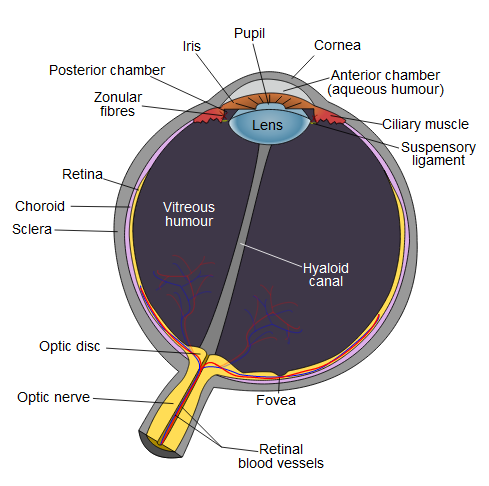
\includegraphics[width=100mm, keepaspectratio]{figures/eye_diagram.png}
\caption{Az emberi szem felépítése. Forrás: \url{http://en.wikipedia.org/wiki/Eye}}
\label{fig:eyediag}
\end{figure}

A \emph{fovea} pozicionálását elősegítő mozgások mellett természetesen más is szerepet kap a kívánt kép előállításában. A teljesség igénye nélkül, ilyenek például a szem divergenciáját illetve konvergenciáját beállító mozgások (mélységérzékelés), valamint azok a reflexszerű mozgások, amelyek az egyensúlyszervvel összhangban beállítják a szemeket a fej térbeli orientációjának megfelelően.

\bigskip

A szakasz első részében sorra veszem, és bemutatom a pozicionáló típusú szemmozgások alapjait, a mérnöki megközelítésből jelentéktelen részleteket mellőzve. Végül a \sectref{mozg_osszegzes} szakaszban összefoglalom a megszerzett ismereteket, valamint hogy a megismert mozgások milyen követelményeket, illetve korlátozásokat támasztanak a realizálandó rendszer tervezése során.

%,,,,,,,,,,,,,,,,,,,,,,,,,,,,,,,,,,,,,,,,,,,,,,,,,,,,,,,,,,,,,,,,,,,,,,,,,,,,
\subsection{Szakkádok}\label{sect:szakkadok}
%,,,,,,,,,,,,,,,,,,,,,,,,,,,,,,,,,,,,,,,,,,,,,,,,,,,,,,,,,,,,,,,,,,,,,,,,,,,,

A szakkád mindkét szem gyors, egyidejű, azonos irányú mozgását jelenti. Célja a fixáció áthelyezése az egyik tárgyról a másikra. A mozgás során észlelt jellegzetes ,,ugráló'' mintáról kapta a nevét: a francia \emph{saccader} szó jelentése ,,rángatás'', ,,ugrás''.

A szakkádok lehetnek akaratlagosak és reflexszerűek is. Az egyensúlyszervből érkező jelre például reflexszerűen aktiválódhatnak, míg a tekintetünk, figyelmünk áthelyezése nyilvánvalóan akaratlagos cselekedet. Időtartamban a szakkádok körülbelül 10 és 100~ms közé tehetők. Ez kellően rövid ahhoz, hogy az agy a gyakorlatban ne észlelje, hogy a mozgás alatt nem történik információfelvétel -- vagyis a szakkádikus mozgás közben pár pillanatra effektíve vakok vagyunk. \cite{shebilske}

A szakkádok végrehajtásáról megoszlanak a vélemények. Korábban a szakkádokat ballisztikusnak tartották, vagyis amint a következő fixációs pont helye kiszámításra kerül (nagyjából 200~ms idő alatt), a mozgás már nem megszakítható vagy megváltoztatható. \cite{carpenter_book} Ezt a feltevést támasztotta alá a tény, hogy a végrehajtás 10-100~ms-os időtartama alatt vizuális visszacsatolásra nincs elegendő idő. Léteznek feltevések azonban, amelyek szerint nincs szükség vizuális visszacsatolásra a végrehajtás közbeni megváltoztatáshoz, így a mozgás ballisztikussága (a nagy sebességek miatt) csak látszólagos. \cite{zee}

%,,,,,,,,,,,,,,,,,,,,,,,,,,,,,,,,,,,,,,,,,,,,,,,,,,,,,,,,,,,,,,,,,,,,,,,,,,,,
\subsection{Lassú követések}\label{sect:lassukovetes}
%,,,,,,,,,,,,,,,,,,,,,,,,,,,,,,,,,,,,,,,,,,,,,,,,,,,,,,,,,,,,,,,,,,,,,,,,,,,,

A lassú követés (\emph{smooth pursuit}) mozgó tárgyak vizuális követésére szolgál. Az ilyen típusú mozgás könnyen modellezhető egy negatív visszacsatolású szabályozóval. \cite{carpenter_book}

Egy bizonyos sebességig a szem képes tisztán lassú követést használni a fixáció tárgyon tartására, azonban a 30$^{\circ}$/s sebességnél gyorsabban mozgó tárgyak esetén a megfelelő követéshez általában szakkádok beiktatása szükséges. Itt jegyzendő meg, hogy a lassú követés vízszintes és függőleges irányban nem szimmetrikus: a legtöbb ember a vízszintes mozgásokat jobban, míg a függőleges mozgásokat kevésbé tudja lekövetni (ahol ,,jó'' követésen azt értjük, hogy nem szükséges szakkádok beiktatása). A szakkádokkal ellentétben a lassú követést egyértelműen megváltoztathatja az érzékelt vizuális visszacsatolás, a mozgás nem ballisztikus.

Érdekesség, hogy a legtöbben vizuális stimuláció (tényleges mozgó tárgy) nélkül nem tudnak lassú követéses szemmozgást előidézni, csak rövid szakkádok gyors egymásutánját. Szintén megemlítendő, hogy a lassú követés bár hasonlónak tűnik ahhoz, amikor a fej mozgását ,,kompenzálva'' egy álló tárgy képét fixáljuk a látómezőn, a két mozgás alapvetően különbözik: már abban is, hogy míg az egyik akaratlagos, a másik reflexszerűen hajtódik végre.

%,,,,,,,,,,,,,,,,,,,,,,,,,,,,,,,,,,,,,,,,,,,,,,,,,,,,,,,,,,,,,,,,,,,,,,,,,,,,
\subsection{Fixációk}\label{sect:fixaciok}
%,,,,,,,,,,,,,,,,,,,,,,,,,,,,,,,,,,,,,,,,,,,,,,,,,,,,,,,,,,,,,,,,,,,,,,,,,,,,

A fixációs mozgások a retina stabilizálására szolgálnak, aminek köszönhetően az álló objektumokat tudjuk figyelmünk középpontjában tartani. Az előző szakasz alapján azt gondolhatnánk, hogy a fixációt ugyanazok az idegi pályák aktiválhatják, mint amelyek a lassú követésért felelősek, mindössze a ,,mozgás'' sebessége zérus.

A fixáció azonban több, mint nulla sebességű mozgás: a fixációk közben \emph{tremor}, \emph{drift} és \emph{mikroszakkád} jellegű mozgások váltják folyamatosan egymást. Az állandó mozgást a fényérzékelő sejtek felépítése indokolja. Ha a kép pár másodpercnél tovább marad teljesen változatlanul a retinán, a sejtek telítésbe kerülnek, és a tekintet elhomályosul.

%,,,,,,,,,,,,,,,,,,,,,,,,,,,,,,,,,,,,,,,,,,,,,,,,,,,,,,,,,,,,,,,,,,,,,,,,,,,,
\subsection{Nystagmus}\label{sect:nystagmus}
%,,,,,,,,,,,,,,,,,,,,,,,,,,,,,,,,,,,,,,,,,,,,,,,,,,,,,,,,,,,,,,,,,,,,,,,,,,,,

A nystagmus szakkádok és lassú követések egymásutánja, nem akaratlagos szemmozgás. Előidéződhet optokinetikus úton, illetve patológiásan is (pl. kábítószer-használat hatására). Patológiás nystagmus jelenléte orvosi szempontból lehet jóindulatú, de akár mélyebb neurológiai problémákra is utalhat.

%,,,,,,,,,,,,,,,,,,,,,,,,,,,,,,,,,,,,,,,,,,,,,,,,,,,,,,,,,,,,,,,,,,,,,,,,,,,,
\subsection{Összegzés}\label{sect:mozg_osszegzes}
%,,,,,,,,,,,,,,,,,,,,,,,,,,,,,,,,,,,,,,,,,,,,,,,,,,,,,,,,,,,,,,,,,,,,,,,,,,,,

A fejezet első szakaszában röviden bemutattam a \emph{fovea} pozicionálására szolgáló szemmozgásokat, amelyek alapszintű megismerése elengedhetetlen a tekintetkövető rendszer fejlesztése során. A rendszernek -- ahogy ez a mozgások tulajdonságaiból kitűnik -- mind a gyorsaság, mind a pontosság tekintetében komoly követelményeket kell teljesítenie.

Az elérendő \textit{gyorsasághoz} a szakkádok, mint a leggyorsabb sebességű mozgások időtartama (10-100~ms) adhat támpontot. Egy átlagos kamerakép 60~Hz-es frissítése legjobb esetben 16~ms időközönkénti vizsgálatot tesz lehetővé. Ez az eredmény egy tipikus drágább, digitális webkamera 30 képkocka/másodperces képfrissítésével máris 33~ms-ra csökken, nem is beszélve a 30~FPS-nél gyengébb teljesítményű kamerákról. Tisztában kell lennünk tehát azzal, hogy átlagos képrögzítő hardver használatával előfordulhat olyan szituáció, hogy fizikailag képtelenek vagyunk a nagyon gyors szakkádok pontos követésére.

A \textit{pontosság} tekintetében azt kell figyelembe vennünk, hogy (pl. olvasásnál) a két egymást követő fixációs pont közti eltérés akár szögperces nagyságrendű is lehet. Ezek korrekt elkülönítéséhez nyilvánvalóan minél nagyobb felbontás szükséges. Minél kisebb felbontásúak a felvételek (azaz a szem, illetve a pupilla megjelenítésére relatíve kevesebb képpont kerül), annál nagyobb elmozdulás jut egyetlen képpontra, ami a feldolgozás során a legkisebb elkülöníthető egység.


%,,,,,,,,,,,,,,,,,,,,,,,,,,,,,,,,,,,,,,,,,,,,,,,,,,,,,,,,,,,,,,,,,,,,,,,,,,,,
\section{Optikai megfontolások}\label{sect:hw_optikai}
%,,,,,,,,,,,,,,,,,,,,,,,,,,,,,,,,,,,,,,,,,,,,,,,,,,,,,,,,,,,,,,,,,,,,,,,,,,,,

Az optikai megfontolások közül az első a tekintetkövetés során felhasznált fénytartomány, ami lehet a látható fény tartománya, valamint az infratartomány. A második fontos szempont pedig a kamera látószöge, ami alapjaiban határozza meg a felhasználótól megkívánt beavatkozás mértékét, valamint a szem felbontását (ezzel közvetve az elérhető maximális pontosságot).

\bigskip

A \textbf{látható fényben} történő követés egyértelmű előnye, hogy nem igényel speciális hardvert, a legtöbb, a piacon kapható analóg vagy digitális (web)kamera ebben a tartományban ,,lát''. Sőt, a digitális eszközökben a CMOS/CCD érzékelő elé szinte minden esetben ún. infratükröt (felülvágó szűrőt, amely kirekeszti a látható fény feletti spektrumot) helyeznek, ezeket az eszközöket tehát sikerrel csak látható fényben használhatjuk. A látható fény használatakor azonban nem feledkezhetünk meg annak hátrányairól sem: a követéshez analizálandó kép meglehetősen érzékeny lesz a megfelelő megvilágításra. A fényviszonyok változásának kiküszöbölése komolyabb előfeldolgozást kíván, és extrém esetekben nem is mindig teljesíthető.

\begin{figure}[!ht]
\centering
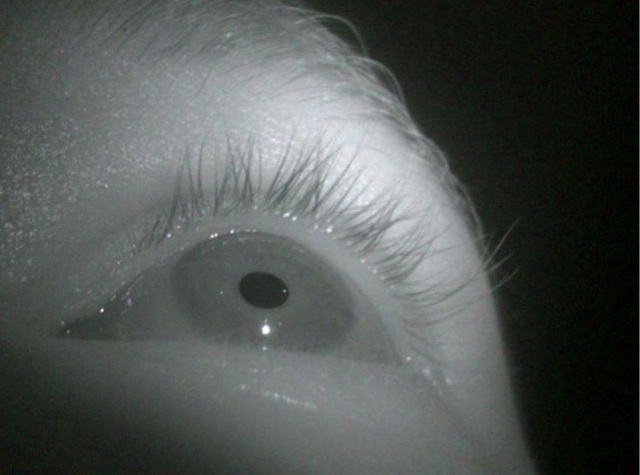
\includegraphics[width=100mm, keepaspectratio]{figures/infra_eye.png}
\caption{Az emberi szem képe infravörös fényben. Forrás: \url{http://bit.ly/aKwzsZ}}
\label{fig:eyepic}
\end{figure}

Az \textbf{infratartománynak} a látható fénnyel szemben vannak előnyei, és hátrányai is. Az előnyök közé tartozik, hogy a pupilla képe a infra megvilágításban nagyon kontrasztos (lásd \figref{eyepic} ábra), jóval könnyebben szegmentálható az írisztől (különösen sötétebb szemű alany esetén), mint látható fényben. Az infrás megvalósítás hátránya azonban, hogy a megfelelő működéshez sötétet igényel (igaz, ezzel összhangban a látható megvilágítási változásokra invariáns), de sötétben, a tisztán infra megvilágítás megvalósítása nehéz feladat, különösen a piacon kapható egyszerűbb infra LED-ekkel, vagy LED-es reflektorokkal.

\bigskip

A követéshez használt kamera optikája lehet egyrészt \textbf{nagylátószögű}. Ez azzal az előnnyel jár, hogy a vizsgálat alatt álló személy fejmozgása szabadabb lehet, nincs szükség a fejpozíció fixálására (pl. álltámasszal). A szemrégió külön szegmentálható, majd ezen régión belül a pupillát követve valósulhat meg a tekintetkövetés. A módszer hátránya, hogy a szemrégió nem tölti be az egész képet, vagyis nem használja ki maximálisan a rendelkezésre álló felbontást. Ennek következtében a tekintetkövetés pontossága jelentős mértékben romolhat, esetleg lehetetlenné is válhat.

További lehetőség a \textbf{teleobjektívek}, vagyis zoomoptikák használata. Teleobjektívvel a szemrégió ,,közel hozható'' még nagy távolságról is, hogy teljesen kitöltse a feldolgozandó képet, kihasználva annak teljes felbontását. Ez azonban azzal a hátránnyal jár, hogy a fejet fix pozícióba kell kényszeríteni (pl. egy álltámasz segítségével), ugyanis a fej mozgásával a pupillarégió kikerülhet a kamera látószögéből.

Végül lehetőség nyílik egyfajta ,,hibrid'' megoldás használatára is, amelynél a két megoldás előnyeit ötvözhetjük.